%%%%%%%%%%%%%%%%%%%%%%%%%%%%%%%%%%%%%%%%%%%%%%%%%%%%%%%%%%%%%%%%%%%%%%%%%%%%%%%%
%2345678901234567890123456789012345678901234567890123456789012345678901234567890
%        1         2         3         4         5         6         7         8

%\documentclass[letterpaper, 10 pt, conference]{ieeeconf}  % Comment this line out
                                                          % if you need a4paper
\documentclass[a4paper, 10pt, conference]{ieeeconf}      % Use this line for a4
                                                          % paper

\IEEEoverridecommandlockouts                              % This command is only
                                                          % needed if you want to
                                                          % use the \thanks command
\overrideIEEEmargins

\usepackage{epsf,graphicx}
\usepackage{latexsym,amssymb}
\usepackage{setspace,cite}
\usepackage{parskip}
\usepackage{amsmath}
\usepackage{amssymb}
\usepackage{listings}
\usepackage{color}
\usepackage{xcolor}
\usepackage{float}
\usepackage{graphicx}
\usepackage[bookmarks=true,pdfborder={0 0 0}]{hyperref}
\usepackage{subcaption}
\usepackage{tensor}
\usepackage{lscape}
%\usepackage[export]{adjustbox}
%\usepackage{mdframed}
\usepackage{textcomp}
\providecommand{\e}[1]{\ensuremath{10^{#1}}}
%\allowdisplaybreaks%%%

\title{\LARGE \bf
Visual Servoing Using Trifocal Tensor
}

\author{\IEEEauthorblockN{Marwan Osman}
  \IEEEauthorblockA{University of Burgundy\\
    71200 Le Creusot, France\\
    email: marwan.aosman@gmail.com}% <-this % stops a space
\and
\IEEEauthorblockN{Fran\c{c}ois Chaumette}
\IEEEauthorblockA{INRIA Rennes-Bretagne Atlantique and IRISA\\
  35042 Rennes, France\\
  email: francois.Chaumette@irisa.fr}
}

\author{ \parbox{3 in}{\centering Marwan Osman\\
         University of Burgundy\\
         71200 Le Creusot, France\\
         {\tt\small marwan.aosman@gmail.com}}
         \hspace*{ 0.5 in}
         \parbox{3 in}{ \centering Fran\c{c}ois Chaumette\\
          INRIA Rennes-Bretagne Atlantique and IRISA\\
         35042 Rennes, France\\
         {\tt\small francois.Chaumette@irisa.fr}}
}

\begin{document}
\maketitle
\thispagestyle{empty}
\pagestyle{empty}

%%%%%%%%%%%%%%%%%%%%%%%%%%%%%%%%%%%%%%%%%%%%%%%%%%%%%%%%%%%%%%%%%%%%%%%%%%%%%%%%
\begin{abstract}
Visual servoing is an approach for controlling the motion of a robotic system from visual measurements. Many works have been realized in the past in this area, and is mainly divided into two main categories: Image-based, and Pose-based Visual Servoing. The trifocal tensor is well known in computer vision for tracing geometric information from three images of the same scene. The purpose of this thesis is to design a visual servoing method of a 6-DOF robot based on the trifocal tensor coefficients. Few studies where conducted on this area but they didn't provide a generic analytical solution for 6-DOF robots. This method differs than the two main visual servoing approaches as the control loop is closed over projective measures, which are the trifocal tensor elements. These projective measures are found directly from images across three views, without explicitly recovering the camera pose or directly closing the loop in the image space. The trifocal tensor geometric model is more robust than the two view geometry models as it involves the information given by a third view, and the set of correspondences obtained is more robust to outliers.
\end{abstract}

\section{INTRODUCTION}
Visual Servoing is a growing active field of research. Recent advances in robotics and computer vision domains has led to the emergence of this vision-based closed loop control methods to control a robot manipulator or a mobile robot through vision acquired by a camera. Many works have studied closing the control loop over visual features computed either from the image space (IBVS) or the estimated 3D pose of the scene (PBVS). There exist some approaches which cannot be considered part of the main two classes of Visual Servoing approaches IBVS and PBVS. These approaches differ than the two main visual servoing classes by closing the control loop over projective measures, which are not computed directly from the image space or the 3D pose. Epipolar geometry can be used to estimate depth, which appears in the interaction matrix of point features\cite{malis20002}. Chesi \textit{et al.} controlled a holonomic mobile robot from a partially calibrated camera using the symmetry of epipolar geometry without point correspondences \cite{chesi}. Benhimane and Malis developed a homography-based approach without reconstructing any 3D parameters \cite{Malis}. Lopez-Nicolas \textit{et al.} designed a homography-based controller which considers the non-holonomic constraints \cite{lopez2006}. These methods use the two-view geometry between the observed and desired views and ignore their relation with the initial view. Epipolar geometry is not well-conditioned if the features are coplanar or the baseline is short, while homography-based approaches require dominant planes.

Recent works introduced using the three-views geometry in the visual servoing loop. The trifocal tensor encapsulates the intrinsic geometry between the three views, and It is analogous for the fundamental matrix in stereo vision systems. The trifocal tensor geometric model is more robust than the two view geometry models as it involves the information given by a third view, and the set of correspondences obtained is more robust to outliers. The application of trifocal tensor in visual servoing has been neglected until recently. Becerra and Sagues used a simplified trifocal tensor as measurement and estimate and track the pose of a non-holonomic mobile robot with Extended Kalman Filter (EKF) \cite{becerra2009pose}. Lopez-Nicolas \textit{et al.} used the constrained camera motion on a mobile robot and linearized the input-output space for control \cite{lopez2010visual}. This approach provided an analytical interaction matrix, which relates the variations of 9 elements of the trifocal tensor to the motion velocities. Shademan used the trifocal tensor for 6-DOF visual servoing \cite{shademan2010three}. Unlike Lopez-Nicolas, Shademan didn't provide an analytical derivation for the interaction matrix, it was estimated numerically and used in the control law. Shademan argued that using the trifocal tensor to control 6-DOF visual servoing loop was not introduced prior to his work due to the difficulty in linearizing the input-output space in the case of the generalized 6-DOF camera motions.

The work of this paper is based on the previous approaches introduced by Lopez-Nicolas \cite{lopez2010visual} and Shademan \cite{shademan2010three}. An approach to incorporate the trifocal tensor estimated from the three-views geometry into the visual servoing control loop task has been presented in this work. This approach presents a generalized 6-DOF visual servoing task, with the control loop being closed over projective measures, namely the trifocal tensor coefficients. To the best of our knowledge, this approach is the first to propose a fully analytical design for a visual servoing task based on the trifocal tensor. First, we present brief background on the Trifocal Tensor and Visual Servoing. Next, we present the analytical development of the new approach. We discuss the obtained results. Finally, we present an overall conclusion fo the work in hand, as well as possible improvements and future work.

\section{BACKGROUND}
\subsection{Trifocal Tensor}
The Trifocal Tensor is a $3 \times 3 \times 3$ array of numbers that incorporates all projective geometric relationships among three views \cite{Hartley2004}. It relates the coordinates of corresponding points or lines in three views, being independent of the scene structure and depending only on the relative pose among the three views and their intrinsic calibration parameters. In this method, we assume the camera intrinsic parameters are known. It means before computing the tensor from image correspondences, matching points have to be transformed to calibrated coordinates. The geometric basis for the trifocal tensor can be deduced from the incidence relationship of three corresponding lines projecting a line in 3D-space. The computation is described in details in \cite{Hartley2004}. Let the Camera positions be $C_{c^*},C_c,C_i$ for the desired, current, and initial camera positions respectively. And their projection matrices be $[I | 0]$, $[ ^{c}{\bf R}_{c^*} | ^{c}{\bf t}_{c^*} ]$, $[ ^{i}{\bf R}_{c^*} | ^{i}{\bf t}_{c^*} ]$. The Tensor relation can then be expressed as follows
\begin{equation}
\mathcal{T}_{(jkl)} = \tensor[^{c}]{R}{_{c^{*}(kj)}} \ \tensor[^{i}]{t}{_{c^{*}(l)}} - \tensor[^{c}]{t}{_{c^{*}(k)}} \ \tensor[^{i}]{R}{_{c^{*}(lj)}} \label{eq:tensorcoeffs}
\end{equation}

\begin{figure}[ht!]
  \centering
  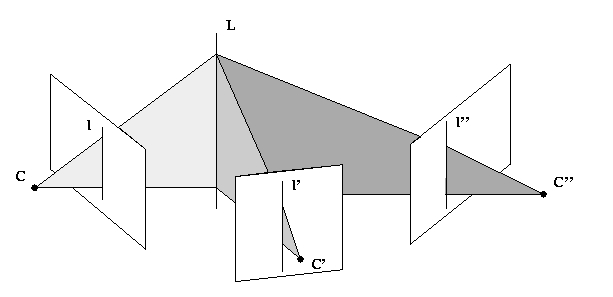
\includegraphics[width=80mm]{figures/threeviews.jpg}
  \caption{Trifocal geometry of three views}
  \label{fig:threeviews}
\end{figure}

$\mathcal{T}$ is then the trifocal tensor relating the 3 views together. It has 27 elements. There are 26 independent rations apart from the common overall scaling factor of the tensor. However, the tensor has only 18 independent parameters. Each of the three camera projection matrices has 11 parameters which makes $33$ in total. However, $15$ parameters must be subtracted to account for the projective world frame, thus leaving 18 parameters.

Since the trifocal tensor embeds the geometry of the three cameras in the scene, this implies that the camera matrices may be computed from the trifocal tensor up to a projective ambiguity~\cite{Hartley2004}. First, the epipoles $e^{\prime},e^{\prime \prime}$ are retrieved. Let $u_i$ and $v_i$ be the left and right null-vectors respectively of $\mathcal{T}_{i}$, \textit{i.e.:} $u_{i}^{T} \mathcal{T}_{i} = {\bf 0}^{T}, \mathcal{T}_{i}v_i = 0$. Then the epipoles are obtained as the null vectors of the following $ 3 \times 3$ matrices:
\begin{equation}
  e^{\prime T} [u_1, u_2, u_3] = 0  \text{ and } e^{\prime \prime T}[v_1, v_2, v_3] = 0
  \label{eq:recoveringepipoles}
\end{equation}
Next, to retrieve the camera matrices $P^{\prime}, P^{\prime \prime}$, the epipoles are first normalized to unit norm, and we have:
\begin{equation}
\begin{gathered}
  P^{\prime} = [[\mathcal{T}_{1}, \mathcal{T}_{2},\mathcal{T}_{3}] e^{\prime \prime} | e^{\prime}] \text{ and }\\ P^{\prime \prime} = [(e^{\prime \prime} e^{\prime \prime T} - I)[\mathcal{T}_{1}^{T}, \mathcal{T}_{2}^{T},\mathcal{T}_{3}^{T}] e^{\prime} | e^{\prime \prime}]
  \end{gathered}\label{eq:recoveringprojectionmatrices}
\end{equation}
The trifocal tensor can be computed from feature correspondences across the three views. Computation of tensor using correspondences of points or lines has been studied extensively in literature. The main linear algorithm presented by \texttt{Hartley}\cite{Hartley2004} is the straightforward method to compute the tensor. Other methods make use of \texttt{RANSAC} (RANdom SAmple Consensus) to enable the tensor estimation to be robust to outliers that usually cause the linear algebraic method to fail \cite{torr1997robust}.
Each triplet of corresponding image points gives 4 equations linearly independent. Therefore, a minimum set of 7 correspondences of non-planar points are needed for the trifocal tensor computation to uniquely determine the 27 entries of the tensor matrix. This method suffers from two issues however: the tensor is parameterized by all its entries and this does not take into account the tensor geometrical constraints, therefore, there is always a risk of obtaining an invalid tensor; and, using all available point correspondences causes the tensor to be significantly affected by the presence of strong outliers.
Hence, an algebraic minimization is needed there after, to use the linear solution as an initial estimate and re-parameterize it by the 24 entries of the projection matrices $P^\prime$ and $P^{\prime \prime}$. The desired tensor is found by minimizing the residual error. The latter algorithm leads to a geometrically valid tensor. However, the main weakness of the algebraic minimization method is that all point correspondences are involved in the tensor computation and still suffers from outliers in practice.
%%%%%%%%%%%%%%%%%%%%%%%%%%%%%%%%%%%%%%%%%%%%%%%%%%%%%%%%%%%%%%%%%%%%%%%%%%%%%%%%%%%%%%%%%%%%%%
\subsection{Visual Servoing}
Visual Servoing refers to the family of closed loop control techniques to control the degrees of freedom of an actuated system with visual feedback\cite{chaumette2006visual}. The vision data may be acquired from a camera that is mounted directly on the robot, or the camera can be fixed in the workspace so that it can observe the robot motion from a stationary configuration. The goal of many robotic applications is to place the robot at a desired configuration to manipulate an object in the environment. The objective of closed loop control techniques is to minimize an error function $e(t)$ defined as
\begin{equation}
  e(t) = s(t) - s^{*}
  \label{eq:servo1}
\end{equation}
where $s$ is a vector of visual features, and the vector $s^*$ has the desired values of these features at the desired configuration.

Then, to design the control scheme, the relationship between the time variation of the features $s$ and the camera velocity has to be found. Noting the spatial velocity of the camera $u_c = (v_c, \omega_c)$, where $v_c$ is the instantaneous linear velocity of the origin of the camera frame, and $\omega_c$ is the instantaneous angular velocity of the camera frame. The relationship between $\dot{s}$ and $u_c$ is given by
\begin{equation}
  \dot{s} = L_s u_c
  \label{eq:servo2}
\end{equation}
where $L_s$ is called the \textbf{interaction matrix} related to $s$. This matrix relates the rate of changes of the image feature velocities $\dot{s}$ to the rate of change of the pose parameters which is the camera velocity. From~\eqref{eq:servo1} and~\eqref{eq:servo2}, the relationship between the camera velocity and the derivative of the error is
\begin{equation}
  \dot{e} = L_s u_c
\label{eq:servo3}
\end{equation}
Considering $u_c$ as the input to the robot controller, to ensure an exponential decoupled decrease of the error, we would like to have $\dot{e} = -\lambda e$, using~\eqref{eq:servo3} we obtain the following control law equation
\begin{equation}
  u_c = -\lambda L_{s}^{+} e
\label{eq:servo4}
\end{equation}
where $L_{s}^{+}$ is the pseudo-inverse of $L_s$. This is the basic visual servoing closed loop system framework. Different visual servoing approaches differ only in the selection of the visual features $s$ and deriving their corresponding interaction matrices $L_s$.

There are three main classes of visual servoing: Image-based Visual Servoing (IBVS), Pose-based Visual Servoing (PBVS), and Hybrid Visual Servoing (HVS) \cite{chaumette2006visual}\cite{chaumette2007visual}. In IBVS, the features are computed from the 2D image data, while in PBVS, the features are computed from the estimated pose from image measurements. HVS use a combination of 2D and 3D visual features. The choice of the visual features is important and generally affects the performance of the visual servoing system. The IBVS approach is more robust to modeling and measurement noise than PBVS. However, the IBVS approach only guarantees local asymptotic stability. It also suffers from degenerate cases and may fail to reach the goal state. PBVS approach ensure global asymptotic stability if the pose estimation is perfect. The pose estimation algorithm must be realized in real-time to calculate the error at every control iteration, and hence more computationally expensive than IBVS approach. However, PBVS approach is more sensitive to image measurement noise and outliers. It usually also requires full knowledge of the geometric object model, and the camera intrinsic calibration.
%%%%%%%%%%%%%%%%%%%%%%%%%%%%%%%%%%%%%%%%%%%%%%%%%%%%%%%%%%%%%%%%%%%%%%%%%%%%%%%%%%%%%%%%%%%%%%

\section{METHODOLOGY}\label{sec:methodology}
To formulate the control law of the trifocal tensor based visual servoing \eqref{eq:tensorcontrollaw}, we need to establish the model of the system and find the relation between the input of the control and the trifocal tensor coefficients. That is to find the interaction matrix relating the control input and the tensor coefficients derivatives. The error will be the difference between the current tensor and the desired tensor values.
\begin{equation}
  \begin{gathered}
  \dot{\mathcal{T}}_{(jkl)} = L_{\mathcal{T}_{(jkl)}} u_c\\
  u_c = -\lambda L_{\mathcal{T}_{(jkl)}}^{+} e
\end{gathered} \label{eq:tensorcontrollaw}
\end{equation}

\subsection{Interaction Matrix}
First, The derivatives of all the trifocal tensor elements with respect to time are generally as following:
\begin{equation}
  \begin{gathered}
  \dot{\mathcal{T}}_{(jkl)} = \tensor[^{c}]{\dot{R}}{_{c^{*}(kj)}} \tensor[^{i}]{t}{_{c^{*}(l)}} + \tensor[^{c}]{R}{_{c^{*}(kj)}} \tensor[^{i}]{\dot{t}}{_{c^{*}(l)}}\\ - \tensor[^{c}]{\dot{t}}{_{c^{*}(k)}} \tensor[^{i}]{R}{_{c^{*}(lj)}} - \tensor[^{c}]{t}{_{c^{*}(k)}} \tensor[^{i}]{\dot{R}}{_{c^{*}(lj)}} \end{gathered}\label{eq:tensorderivatives1}
\end{equation}

Since our initial camera $C_i$ is fixed, the elements of the derivatives of its rotation matrix and its transpose vector are equal to zero, \textit{i.e.:} $\tensor[^i]{\dot{t}}{_{c^{*}(l)}} = \tensor[^i]{\dot{R}}{_{c^{*}(jl)}} = 0$. Our trifocal tensor elements derivative is then simplified to:
\begin{equation}
  \dot{\mathcal{T}}_{(jkl)} = \tensor[^{c}]{\dot{R}}{_{c^{*}(kj)}} \ \tensor[^{i}]{t}{_{c^{*}(l)}} - \tensor[^{c}]{\dot{t}}{_{c^{*}(k)}} \ \tensor[^{i}]{R}{_{c^{*}(lj)}} \label{eq:tensorderivatives2}
\end{equation}

The spatial velocity of the camera is $u_c = {(v_c, \omega_{c})}^{T}$, where $v_c$ and $\omega_c$ are the translational and rotational velocities of the camera. From the geometry of the scene, we can deduce the following relationships:
\begin{gather*}
  {[\omega_{c}]}_{\times} = \tensor[^{c^*}]{R}{_{c}^{T}} \tensor[^{c^*}]{\dot{R}}{_{c}} = - \tensor[^{c^*}]{\dot{R}}{_{c}^{T}} \tensor[^{c^*}]{R}{_{c}}\\
  \tensor[^{c^*}]{\dot{R}}{_{c}^{T}} = - {[\omega_{c}]}_{\times}\tensor[^{c^*}]{R}{_{c}^{T}}\\
  \tensor[^{c^*}]{\dot{R}}{_{c}^{T}} = - {[\omega_{c}]}_{\times}\tensor[^{c}]{R}{_{c^*}}\\
  \tensor[^{c}]{\dot{R}}{_{c^*}} = -{[\omega_c]}_{\times}\tensor[^{c}]{R}{_{c^*}}
  \end{gather*}
  Similarly, we have \cite{chaumette2006visual}:
  \begin{gather*}
  \tensor[^{c^*}]{\dot{t}}{_{c}} = \tensor[^{c^*}]{R}{_{c}}v_{c}, \tensor[^{c}]{t}{_{c^*}} = - \tensor[^{c}]{R}{_{c^*}} \tensor[^{c^*}]{t}{_{c}}\\
  \tensor[^{c}]{\dot{t}}{_{c^*}} = - \tensor[^{c}]{\dot{R}}{_{c^*}} \tensor[^{c^*}]{t}{_{c}} - \tensor[^{c}]{R}{_{c^*}} \tensor[^{c^*}]{\dot{t}}{_{c}}\\
  \tensor[^{c}]{\dot{t}}{_{c^*}} = {[\omega_c]}_{\times}\tensor[^{c}]{R}{_{c^*}} \tensor[^{c^*}]{t}{_{c}} - \tensor[^{c}]{R}{_{c^*}} \tensor[^{c^*}]{R}{_{c}}v_{c}\\
  \tensor[^{c}]{\dot{t}}{_{c^*}} = {[\omega_c]}_{\times}\tensor[^{c}]{t}{_{c^*}} - v_{c}\\
  \tensor[^{c}]{\dot{t}}{_{c^*}} = {[\tensor[^{c}]{t}{_{c^*}}]}_{\times}\omega_c - v_{c}\\
  \tensor[^{c}]{\dot{t}}{_{c^{*}(k)}} = [-I | {[\tensor[^{c}]{t}{_{c^*}}]}_{\times}] u
\end{gather*}

Substituting back into the tensor derivation \eqref{eq:tensorderivatives2}, we get:
\begin{equation}
\begin{gathered}
  \dot{\mathcal{T}}_{(jkl)} =  - {({[\omega_c]}_{\times}\tensor[^{c}]{R}{_{c^*}})}_{(kj)}\ \tensor[^{i}]{t}{_{c^*(l)}} \\- {({[\tensor[^{c}]{t}{_{c^*}}]}_{\times}\omega_c - v_{c})}_{(k)}\ \tensor[^{i}]{R}{_{c^*(lj)}}\\
  \dot{\mathcal{T}}_{(jkl)} =  - (\sum_{m}{[\omega_{c}]}_{\times(km)}\tensor[^{c}]{R}{_{c^*(mj)}})\ \tensor[^{i}]{t}{_{c^*(l)}} \\- ({({[\tensor[^{c}]{t}{_{c^*}}]}_{\times}\omega_c)}_{(k)}  -   v_{c(k)})\ \tensor[^{i}]{R}{_{c^*(lj)}}
\end{gathered}\label{eq:tensorderivatives3}
\end{equation}

From~\eqref{eq:tensorcoeffs} and~\eqref{eq:tensorderivatives3}, we can compute the derivatives for all the coefficients, and deduce this compact form:
\begin{equation}
  \dot{\mathcal{T}}_{(jkl)} = R_{i(lj)}v_{c(k)} - \sum_{m} {[\omega_{c}]}_{\times(km)} \mathcal{T}_{(jml)}
\label{eq:tensorderivativesgeneral}
\end{equation}

To control the six degrees of freedom, at least six tensor coefficients are necessary. However, to avoid singularities, more than six tensor coefficients are considered. The interaction matrix $L_{T_{(jkl)}}$ taking into account all the tensor coefficients can be deduced from \eqref{eq:tensorderivativesgeneral}. It is important to notice that pose of the initial camera location is necessary for the computation of the interaction matrix as well as the normalization factor. It is also to be noticed there exists a decoupling between the translational velocities in the resulting interaction matrix. This decoupling ensures to obtain smooth camera trajectories for the motion in the 3D space.

\subsection{Tensor Normalization} \label{sub:tensor_normalization}
Since the trifocal tensor is computed up to a scale factor, we propose a normalization step to get a fixed scale. The normaliztion factors $\mathcal{T}_{kN}$ are used to obtain the normalized tensor $T_{jkl}$.  When the camera reaches the desired goal position, we can observe that the tensor coefficients are only related to the translation of the camera at the initial position which is a constant value vector. Also from~\eqref{eq:tensorderivativesgeneral}, the first column elements $\mathcal{T}_{(111)}$, $\mathcal{T}_{(112)}$, $\mathcal{T}_{(113)}$, $\mathcal{T}_{(211)}$, $\mathcal{T}_{(212)}$, $\mathcal{T}_{(213)}$, $\mathcal{T}_{(311)}$, $\mathcal{T}_{(312)}$, $\mathcal{T}_{(313)}$ are respectively equal to $\tensor[^{i}]{t}{_{c^*(1)}}$, $\tensor[^{i}]{t}{_{c^*(2)}}$, $\tensor[^{i}]{t}{_{c^*(3)}}$, $0$,$0$,$0$,$0$,$0$,$0$ at the desired goal position.

Choosing the elements $\mathcal{T}_{(111)}$, $\mathcal{T}_{(112)}$, $\mathcal{T}_{(113)}$ as normalization factors would seem a good choice for our method, as we would be interested in coefficients converging to non-zero values. However, it was found that for some scene configurations, these three coefficients could have values equal to zero at the initial pose. Which means at normalization step, this would cause dividing by a zero value. To avoid this problem, we will use all the nine coefficients of the first column to be our first normalization factor. We can then normalize the elements $T_{jkl}$ for $k = 1$ as follows:
\begin{equation}
  \begin{gathered}
    T_{jkl} = \frac{\mathcal{T}_{jkl}}{\mathcal{T}_{1N}}\\
    \mathcal{T}_{1N} = ({\mathcal{T}_{111}}^{2}+{\mathcal{T}_{112}}^{2}+{\mathcal{T}_{113}}^{2}+{\mathcal{T}_{211}}^{2}+{\mathcal{T}_{212}}^{2}+{\mathcal{T}_{213}}^{2} \\+ {\mathcal{T}_{311}}^{2}+{\mathcal{T}_{312}}^{2}+{\mathcal{T}_{313}}^{2}) ^{\frac{1}{2}}
  \end{gathered}
\end{equation}

Unfortunately, this normalization factor is dependent on the tensor coefficients which varies with time. So we need to find also the derivative of the normalization factor.
A general formula for $\dot{T}_{(jkl)}$ can then be found as following
\begin{equation}
  \begin{gathered}
    \dot{T}_{(jkl)} = \frac{\tensor[^{i}]{R}{_{c^{*}(lj)}}}{\mathcal{T}_{kN}}v_{c(k)} -T_{(jkl)}(\sum_n \sum_{m}T_{nkm}\frac{\tensor[^{i}]{R}{_{c^{*}(mn)}}}{\mathcal{T}_{kN}}) v_{c(k)}\\ + T_{(jkl)}(\sum_n \sum_{m}T_{nkm}T_{nhm})\omega_{(g)} \\- T_{(jkl)}(\sum_n \sum_{m}T_{nkm}T_{ngm})\omega_{(h)} \\+\sum_{m} {[\omega_{c}]}_{\times(km)} T_{(jml)}\\
      \text{where } g = k\%3 +1, h = (k+1)\%3 +1
  \end{gathered}\label{eq:tensornormalizationgeneral}
\end{equation}

From \eqref{eq:tensornormalizationgeneral}, the final normalized interaction matrix can be computed. As we notice, this particular choice for the normalization factors has led to keep the decoupling property between the translational velocities, as each degree of freedom related tensor coefficients are normalized separately from other degrees of freedom. Other choices of different combinations of tensor coefficients as normalization factors, would introduce extra non-zero elements to the normalized interaction matrix and prevent keeping the decoupling property.

\subsection{Proposed Method}
We have defined all the elements of the control law \eqref{eq:tensorcontrollaw}. The interaction matrix $L_{T_{(jkl)}}$ is computed as indicated in \eqref{eq:tensornormalizationgeneral}. The error $e$ is computed using the difference between the current tensor coefficients and the desired tensor coefficients, $e = T_{(jkl)} - T_{(jkl)}^{*}$. In Figure \ref{fig:vsttloop}, we present the block diagram explaining the proposed trifocal tensor visual servoing control loop. At initialization, the desired tensor $T_{(jkl)}^{*}$ is computed from feature correspondences across three images obtained from the three camera poses: initial pose, desired pose, and current pose being equal to the desired pose.
\begin{figure*}[ht!]
  \centering
  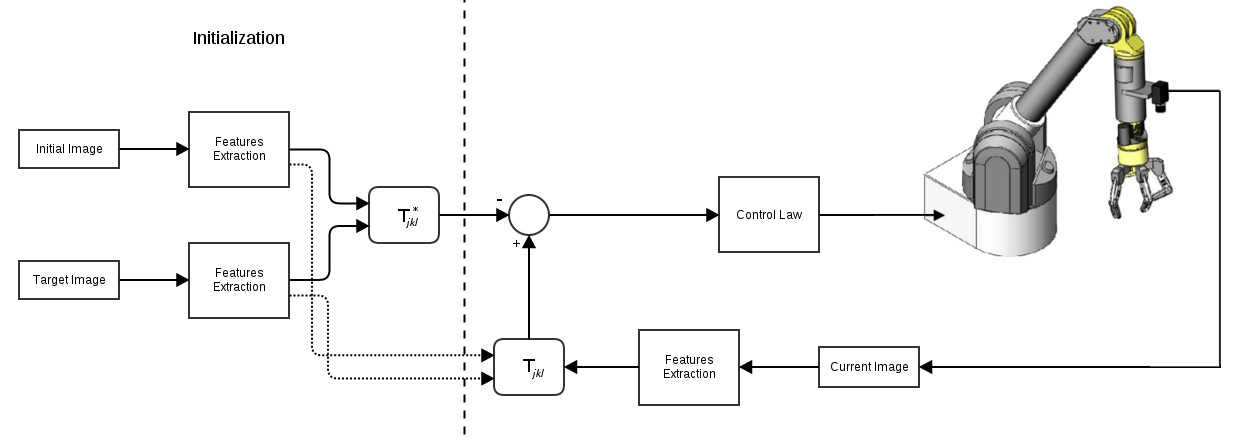
\includegraphics[width=150mm,height=50mm]{figures/vsttloop.png}
  \caption{Block diagram of the proposed Trifocal Tensor Visual Servoing loop control}
  \label{fig:vsttloop}
\end{figure*}

The current tensor $T_{(jkl)}$ is computed inside the visual servoing loop at each iteration. Then the interaction matrix is computed using the current tensor. For simplicity, we make the assumption that the initial pose is known and the interaction matrix can be computed directly. The new error value is computed along with the pseudo-inverse of the interaction matrix and fed back to the control law to compute the required velocities to drive the camera to the desired pose. The system converges and the loop is terminated when the camera reaches the desired pose. This is evaluated when the sum squared of the error reaches a value less than a defined threshold, $1 \times \e{-6}$ for example.

\section{EXPERIMENTAL RESULTS}\label{sec:results}
The proposed method was implemented in C++, using the \texttt{ViSP} library. \texttt{ViSP} is an open-source visual servoing framework library developed by \texttt{INRIA} and written in C++ \cite{visp}. It is a modular cross platform library that allows prototyping and developing applications using visual tracking and visual servoing techniques. The scene setup is defined with two poses for the camera: initial and desired, along with an object to be tracked in the scene. A trifocal tensor requires at least 7 non coplanar points for estimating a tensor. Throughout our experiments, we used two sets of 8 and 12 points. There are no much differences between the results of the two sets because we are not considering points mismatch and outliers throughout the experiments. The following results are for the set of 12 points.

\subsection{Experiment I: Pure Translation along x-axis, or y-axis}
For first experiment, we consider a pure translational motion along one axis. It's the basic test that can be done to ensure the convergence of the control loop. We consider a small translation of $0.1m$ along x-axis, then y-axis. Figure \ref{fig:ex1cvelocity} shows the evolution of the camera velocities, and Figure \ref{fig:ex1cerror} shows the evolution of the trifocal tensor coefficients error. Figure \ref{fig:ex1c} shows the results of estimating the tensor through points correspondences. A translation along y-axis produces similar results.

\begin{figure}[ht!]
\centering
%\begin{mdframed}[linecolor=black!30,backgroundcolor=black!5]
%\begin{adjustbox}{minipage=.8\linewidth,margin=1ex,bgcolor=black!5,margin=0.3pt,bgcolor=black!30,margin=2ex}
  \centering
  \begin{subfigure}{.48\linewidth}
    \centering
    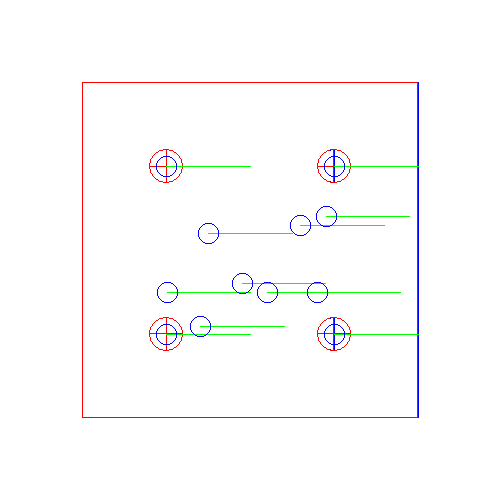
\includegraphics[width=\linewidth]{figures/plots/ex1pimage.png}
    \caption{}
    \label{fig:ex1cimage}
  \end{subfigure}
  \begin{subfigure}{.48\linewidth}
    \centering
    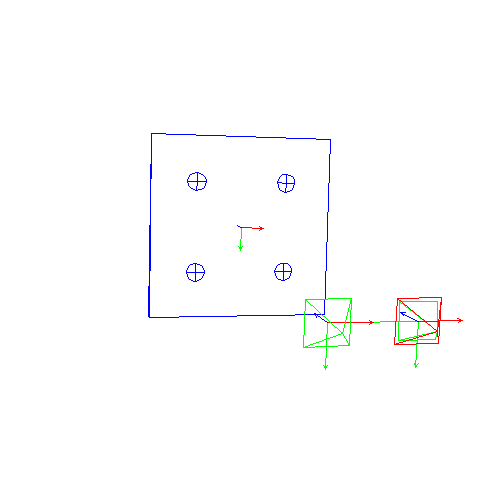
\includegraphics[width=\linewidth]{figures/plots/ex1pscene.png}
    \caption{}
    \label{fig:ex1cscene}
  \end{subfigure}
  \\
  \begin{subfigure}{.48\linewidth}
    \centering
    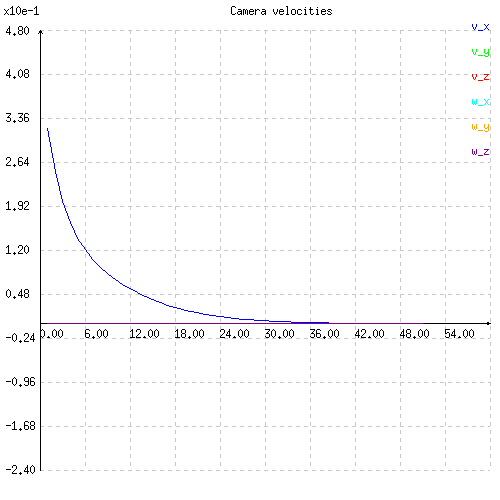
\includegraphics[width=\linewidth]{figures/plots/ex1cvelocity.png}
    \caption{}
    \label{fig:ex1cvelocity}
  \end{subfigure}
  \begin{subfigure}{.48\linewidth}
    \centering
    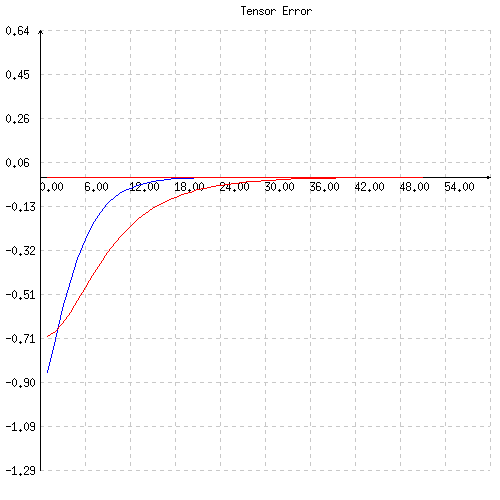
\includegraphics[width=\linewidth]{figures/plots/ex1cerror.png}
    \caption{}
    \label{fig:ex1cerror}
  \end{subfigure}
  \caption{Translation along x-axis using estimated tensor. (a) Image view. (b) Scene view. (c) Camera velocities. (d) Tensor coefficients error.}
  \label{fig:ex1c}
%\end{mdframed}
%\end{adjustbox}
\end{figure}

We observe the camera trajectory is linear, which is satisfactory. However, the error is not exactly exponentially decreasing. Several tests were conducted to analyse the source of this behaviour, and it was found that using a subset of tensor coefficients for computing the error and the interaction matrix leads to a perfect exponentially decreasing error. A subset was chosen experimentally to handle this specific configuration, but different subsets are required for different configurations. Figure \ref{fig:ex1comparison} shows a comparison between the error plots using all the tensor coefficients and using a subset of them.

\begin{figure}[ht!]
\centering
%\begin{adjustbox}{minipage=.9\linewidth,margin=1ex,bgcolor=black!5,margin=0.3pt,bgcolor=black!30,margin=2ex}
  \centering
  \begin{subfigure}{.48\linewidth}
    \centering
    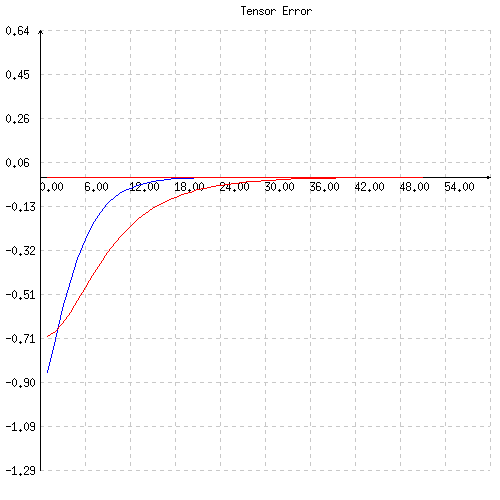
\includegraphics[width=\linewidth]{figures/plots/ex1cerror.png}
    \caption{}
    \label{fig:ex1comparisona}
  \end{subfigure}
  \begin{subfigure}{.48\linewidth}
    \centering
    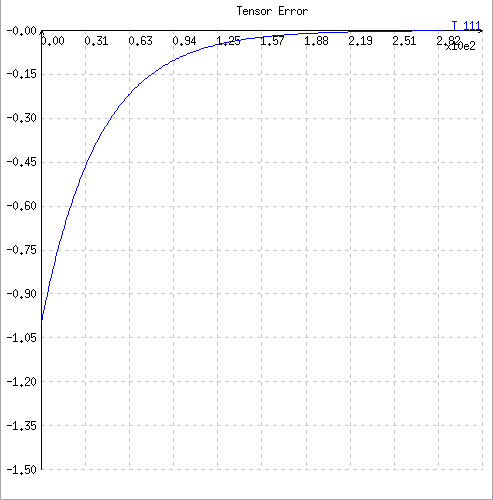
\includegraphics[width=\linewidth]{figures/plots/ex1subset.png}
    \caption{}
    \label{fig:ex1comparisonb}
  \end{subfigure}
  \caption{Comparison between tensor coefficients error when (a) using all tensor coefficients (b) using a subset of tensor coefficients.}
  \label{fig:ex1comparison}
  %\end{adjustbox}
\end{figure}

\subsection{Experiment II: Pure Translation along z-axis}
Motion along the z-axis is usually more challenging than xyz motion in the IBVS approach. This is due to poor motion resolvability when the camera moves towards the feature points \cite{nelson1996vision}. On the contrary, using the trifocal tensor features this motion is not different than other types of motions. Figure \ref{fig:ex2c} show the results for the estimated tensor. Like a simple translation along x-axis or y-axis, a translation along z-axis also suffers the problem of selecting a subset of tensor coefficients.

\begin{figure}[ht!]
\centering
%\begin{mdframed}[linecolor=black!30,backgroundcolor=black!5]
%\begin{adjustbox}{minipage=.8\linewidth,margin=1ex,bgcolor=black!5,margin=0.3pt,bgcolor=black!30,margin=2ex}
  \centering
  \begin{subfigure}{.48\linewidth}
    \centering
    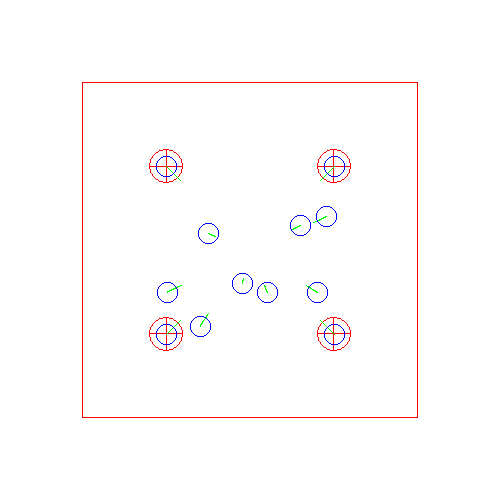
\includegraphics[width=\linewidth]{figures/plots/ex2pimage.png}
    \caption{}
    \label{fig:ex2cimage}
  \end{subfigure}
  \begin{subfigure}{.48\linewidth}
    \centering
    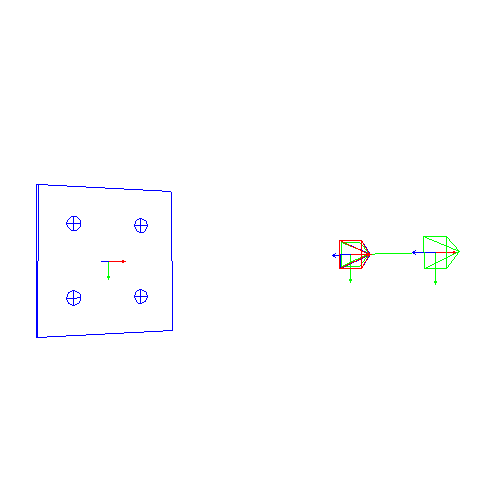
\includegraphics[width=\linewidth]{figures/plots/ex2pscene.png}
    \caption{}
    \label{fig:ex2cscene}
  \end{subfigure}
  \\
  \begin{subfigure}{.48\linewidth}
    \centering
    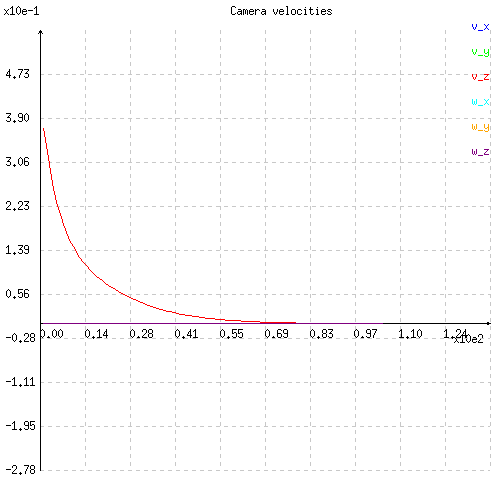
\includegraphics[width=\linewidth]{figures/plots/ex2cvelocity.png}
    \caption{}
    \label{fig:ex2cvelocity}
  \end{subfigure}
  \begin{subfigure}{.48\linewidth}
    \centering
    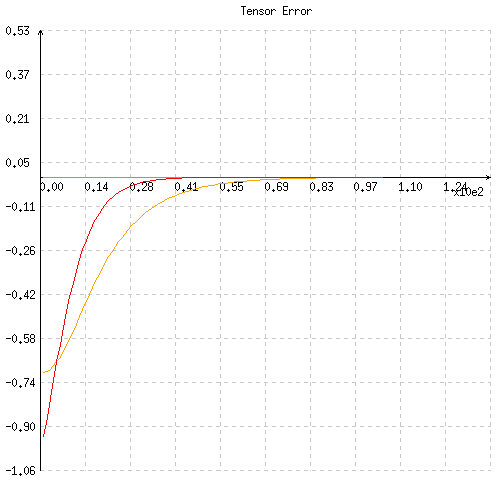
\includegraphics[width=\linewidth]{figures/plots/ex2cerror.png}
    \caption{}
    \label{fig:ex2cerror}
  \end{subfigure}
  \caption{Translation along z-axis using estimated tensor. (a) Image view. (b) Scene view. (c) Camera velocities. (d) Tensor coefficients error.}
  \label{fig:ex2c}
%\end{mdframed}
%\end{adjustbox}
\end{figure}

\subsection{Experiment III: Large rotation around z-axis}
One of the most challenging IBVS configurations is the $180$\textdegree rotation around the z-axis \cite{chaumette2006visual}\cite{chaumette1998potential}. This is due to the nature of the image-based control law which makes the camera retreat from the object instead of rotating around the z-axis. It is important to evaluate the visual servoing method for large z-axis rotations, close to $180$\textdegree.

Here we consider a translation of $1m$ along z-axis and a $170$\textdegree rotation along z-axis. As we can observe in Figure \ref{fig:ex4c}, the retreat problem did not occur. The image trajectories follow a spiral motion, which is exactly as expected due to the linear motion for the translation, and the rotational motion for the rotation.

\begin{figure}[ht!]
\centering
%\begin{mdframed}[linecolor=black!30,backgroundcolor=black!5]
%\begin{adjustbox}{minipage=.8\linewidth,margin=1ex,bgcolor=black!5,margin=0.3pt,bgcolor=black!30,margin=2ex}
  \centering
  \begin{subfigure}{.48\linewidth}
    \centering
    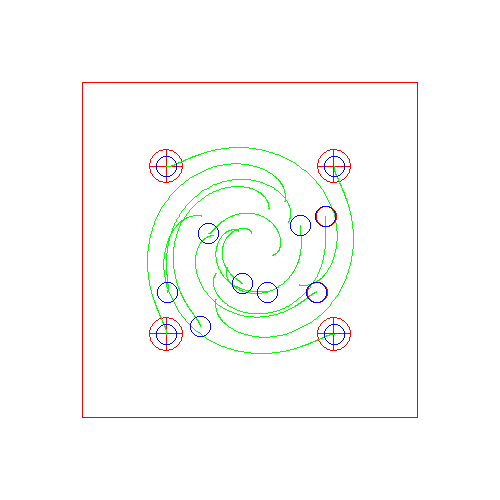
\includegraphics[width=\linewidth]{figures/plots/ex4cimage.png}
    \caption{}
    \label{fig:ex4cimage}
  \end{subfigure}
  \begin{subfigure}{.48\linewidth}
    \centering
    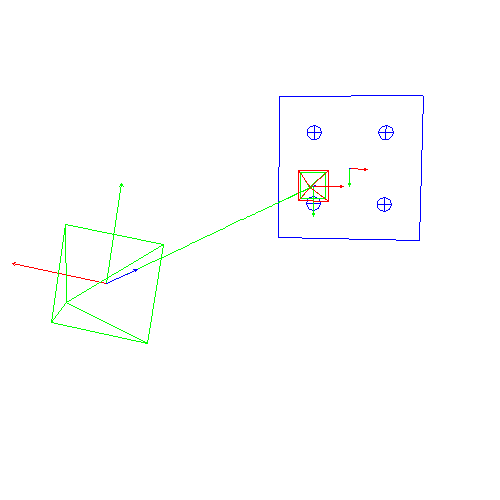
\includegraphics[width=\linewidth]{figures/plots/ex4cscene.png}
    \caption{}
    \label{fig:ex4cscene}
  \end{subfigure}
  \\
  \begin{subfigure}{.48\linewidth}
    \centering
    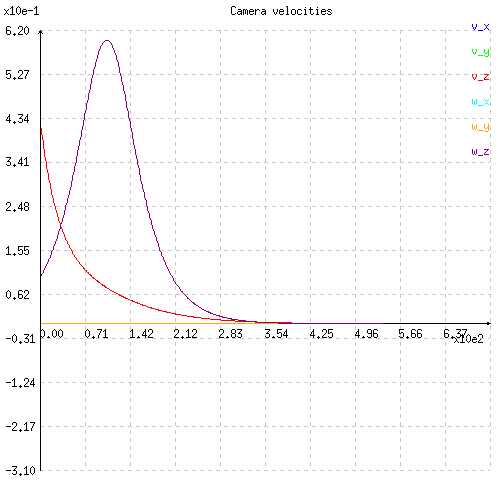
\includegraphics[width=\linewidth]{figures/plots/ex4cvelocity.png}
    \caption{}
    \label{fig:ex4cvelocity}
  \end{subfigure}
  \begin{subfigure}{.48\linewidth}
    \centering
    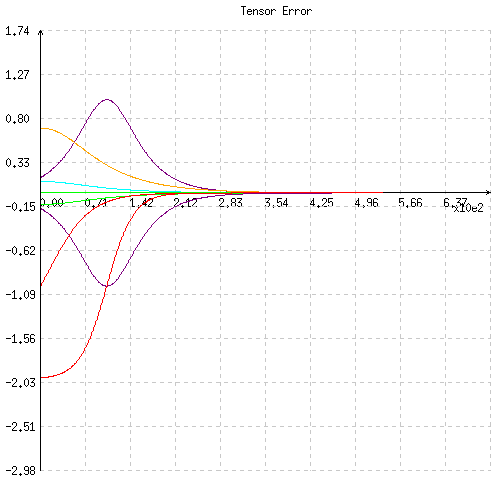
\includegraphics[width=\linewidth]{figures/plots/ex4cerror.png}
    \caption{}
    \label{fig:ex4cerror}
  \end{subfigure}
  \caption{Translation and large rotation along z-axis using estimated tensor. (a) Image view. (b) Scene view. (c) Camera velocities. (d) Tensor coefficients error.}
  \label{fig:ex4c}
%\end{mdframed}
%\end{adjustbox}
\end{figure}

\subsection{Experiment IV: Generic Motion}
In this experiment, we choose a generic camera motion: translations of $0.25m, -03m, 0.2m$, and rotations of $10\text{\textdegree}, -20\text{\textdegree}, 5\text{\textdegree}$ along x,y, and z axes respectively. The results in Figures \ref{fig:ex5c} show smooth camera and image trajectories. However, we notice small oscillations in the camera velocities initially. Lopez-Nicolas \cite{lopez2010visual} mentioned similar oscillations due to noise during image points extraction and matching. Although in our case we omit points mismatch and outliers, this behaviour is most likely due to small numerical error in the trifocal tensor estimation.

\begin{figure}[ht!]
\centering
%\begin{mdframed}[linecolor=black!30,backgroundcolor=black!5]
%\begin{adjustbox}{minipage=.8\linewidth,margin=1ex,bgcolor=black!5,margin=0.3pt,bgcolor=black!30,margin=2ex}
  \centering
  \begin{subfigure}{.48\linewidth}
    \centering
    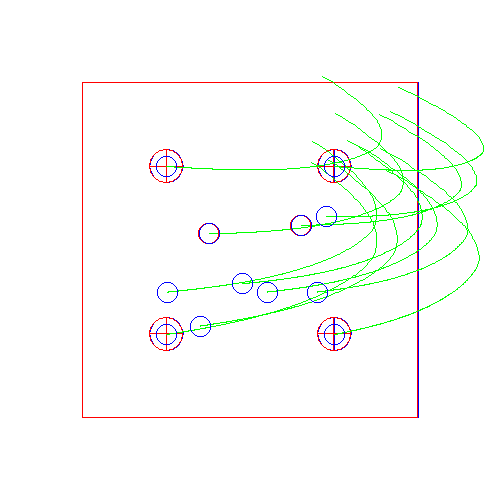
\includegraphics[width=\linewidth]{figures/plots/ex5cimage.png}
    \caption{}
    \label{fig:ex5cimage}
  \end{subfigure}
  \begin{subfigure}{.48\linewidth}
    \centering
    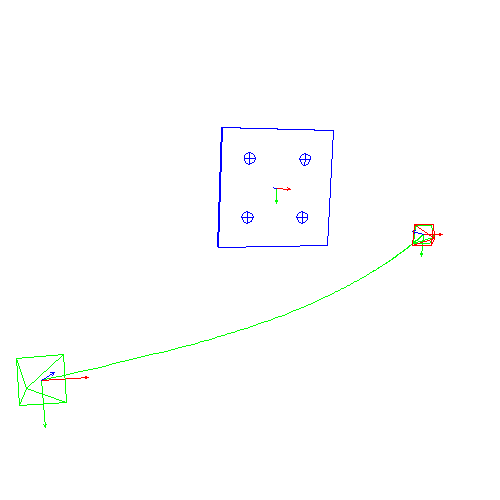
\includegraphics[width=\linewidth]{figures/plots/ex5cscene.png}
    \caption{}
    \label{fig:ex5cscene}
  \end{subfigure}
  \\
  \begin{subfigure}{.48\linewidth}
    \centering
    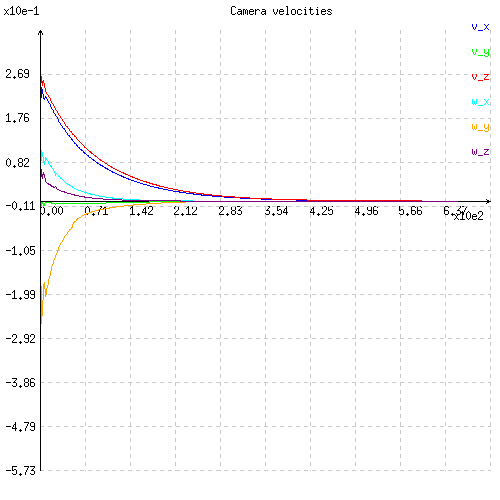
\includegraphics[width=\linewidth]{figures/plots/ex5cvelocity.png}
    \caption{}
    \label{fig:ex5cvelocity}
  \end{subfigure}
  \begin{subfigure}{.48\linewidth}
    \centering
    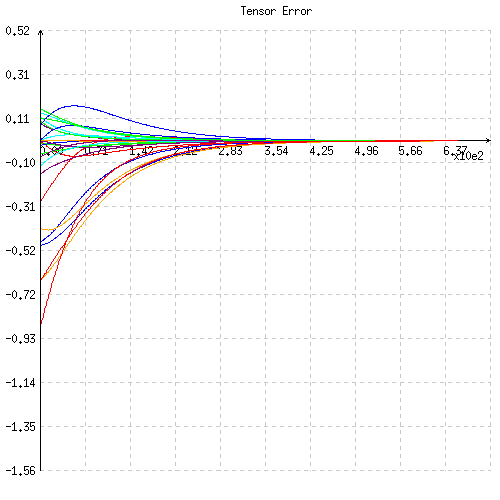
\includegraphics[width=\linewidth]{figures/plots/ex5cerror.png}
    \caption{}
    \label{fig:ex5cerror}
  \end{subfigure}
  \caption{Generic motion using estimated tensor. (a) Image view. (b) Scene view. (c) Camera velocities. (d) Tensor coefficients error.}
  \label{fig:ex5c}
%\end{mdframed}
%\end{adjustbox}
\end{figure}


\section{CONCLUSION and Future Works}
\subsection{Conclusion}

An approach to incorporate the trifocal tensor estimated from the three-views geometry into the visual servoing control loop task has been presented in this work. This approach presents a generalized 6-DOF visual servoing task, with the control loop being closed over projective measures, namely the trifocal tensor coefficients. To the best of our knowledge, this approach is the first to propose a fully analytical design for a visual servoing task based on the trifocal tensor. Previous works either provided an analytical approach for a 3-DOF non-holonomic mobile robot, or provided a full 6-DOF approach but with an interaction matrix estimated numerically rather than analytically.

The experiments showed that this approach is working practically with very satisfactory results. In addition, this approach does not suffer from some of the problems existing in IBVS methods as like the retreat problem.

\subsection{Future Works}
As presented in the section \ref{sec:results}, it was found that using all the trifocal tensor coefficients inside the visual servoing loop does not produce the best results in terms of perfectly exponentially decreasing of the tensor error values. Thus, an automatic optimality selection criteria is needed to dynamically choose the most relevant tensor coefficients. For example, the singular value decomposition of the interaction matrix can reveal which degrees of freedom are most apparent. By selecting features and designing controllers that maximize these measures, the performance of the visual servoing system can be improved. These concepts have been discussed in details in \cite{538976} and \cite{611333}.

Simulation and practical experimentation are not enough for judging the proposed method. We need to prove the existence of only one equilibrium state at the desired pose location. The analysis of the control law can be studied using Lyapunov stability analysis method \cite{spong2006robot}.

We observe in \eqref{eq:tensorderivativesgeneral} that the interaction matrix depends on the knowledge of the initial camera rotation and the normalization factors. In our experimentations, we made an assumption that the initial pose is known from the setup of the simulation. Practically, this information might not be available, and the initial pose needs to be estimated. The initial pose can be retrieved by computing the equivalent projection matrix for the estimated trifocal tensor as shown in~\eqref{eq:recoveringprojectionmatrices}. However, the estimation will still be up to a scale value and not the real value. This scale problem needs to be addressed properly during the tensor normalization step to avoid the scale effects on computing the correct values for the interaction matrix.

The current method assumes the cameras have already been calibrated before-hand. Practically, this may not be the case, so we need to extend the method to cover partially or totally uncalibrated cameras. The introduction of the camera intrinsic parameters matrix $K$ into the formulas, will affect the obtained tensor computation, and hence, the corresponding interaction matrix.

%%%%%%%%%%%%%%%%%%%%%%%%%%%%%%%%%%%%%%%%%%%%%%%%%%%%%%%%%%%%%%%%%%%%%%%%%%%%%%%%
\bibliographystyle{IEEEtran}
\nocite{*}
\bibliography{tex/refs}
%\begin{thebibliography}{99}
%\bibitem{c1}
  %Qingmao Hu, Guoyu Qian, Aziz A. and Nowinski W.L., {\it Segmentation of brain from computed tomography head images}, Engineering in Medicine and Biology  Society 27th Annual International Conference, 2005. IEEE-EMBS 2005.
%\end{thebibliography}
\end{document}
